\section{What this leaves SMILify with}

This internship leaves SMILify with a common articulated coordinate space
for morphological variation across body plans; a way to separate geometry,
anatomy, correspondence, and optimisation as independently testable
questions rather than one opaque fitting procedure; and a demonstrated route from
registration to independently validated measurement for selected traits.
The underlying failure mechanisms are not inherently specific to ants,
although their behaviour on other body plans remains to be established
experimentally.

\begin{figure}[!htb]
\centering
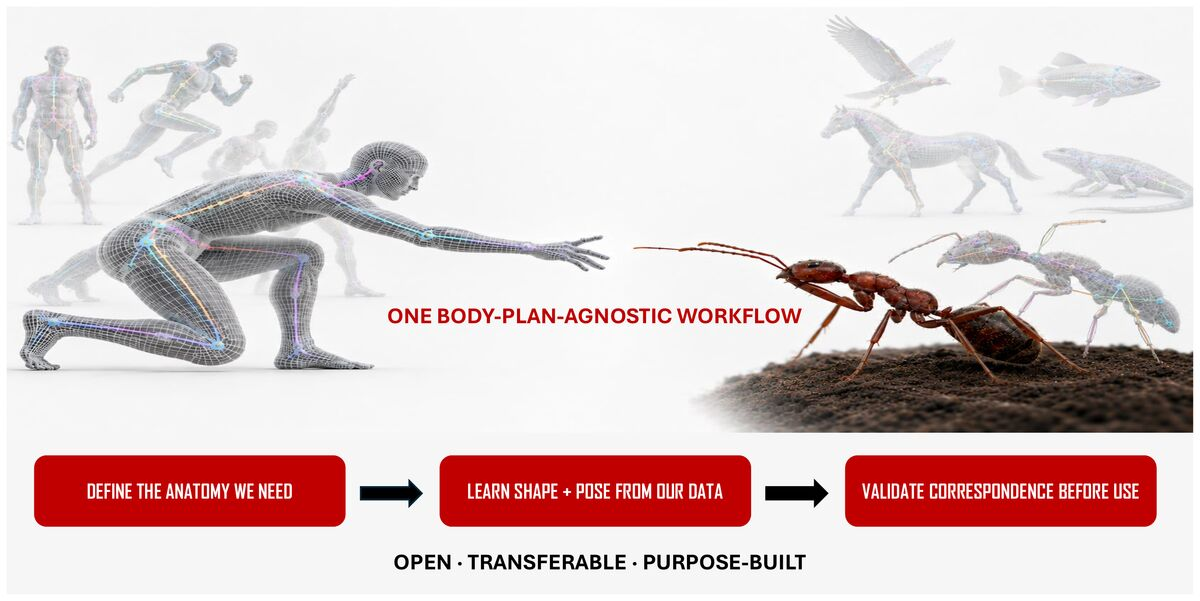
\includegraphics[width=0.6\linewidth]{figures/fig_beyond_ants.jpg}
\caption{The same body-plan-agnostic workflow: define the anatomy,
learn shape and pose from data, validate correspondence before use.}
\label{fig:beyond-ants}
\end{figure}

The workflow this report has diagnosed and partly repaired (define the
anatomy a project needs, learn shape and pose from real data, and validate
correspondence before trusting a single measurement drawn from it;
Figure~\ref{fig:beyond-ants}) was built and tested on ants because that
is where this internship's data and biological questions came from. The
diagnostic framework is designed to generalise beyond the ant case, because
its evaluation levels (surface proximity, anatomical correspondence,
parametric correspondence, and measurement validity;
\S\ref{sec:scale-dependence}) do not depend on a particular number of
limbs or body plan. Whether the specific failure mechanisms found here (a
surface objective with no joint-location term, votes that localise well but
do not deploy densely) recur unchanged on other body plans is an empirical
question this internship's evidence does not settle, and is exactly the
kind of question the same diagnostic framework was built to answer.
